\documentclass[10pt]{article}
\usepackage[margin=0.72in]{geometry}
\usepackage{amsmath,amssymb,graphicx,booktabs,xcolor,hyperref}
\definecolor{ink}{HTML}{253C59}
\hypersetup{colorlinks=true,urlcolor=ink,linkcolor=ink}
\setlength{\parindent}{0pt}\setlength{\parskip}{6pt}
\begin{document}
{\Large\bfseries\color{ink} Native compact spectra for Curve25519}\par
{\small 23 November 2026 \quad Fixed correctness component; unknown-root discovery next}

\textbf{Implemented.} A separate Rust compiler takes public parameters,
$R$, $Q=[8]R$ and a node cap. It builds a monic sextic $S(c)$ from five
unknown normalized coefficients and imposes
\[
 g=T_q\!\left(\frac{A}{2X+A}\right)^2\ \text{in }\mathbb F_p[X]/S,
 \qquad \chi_g(T)=\prod_{i=1}^6\bigl(T-\operatorname{Re}((h^q)^{j_i})^2\bigr).
\]
Map, rational-torsion and squarefree inverse guards stay explicit. Six unknown
labels have $1\le j_i\le k$; repeated coset labels are permitted. Boolean
label/slack words use the explicit field no-wrap premise. All gates and output
constraints survive in the complete SMT export. Newton traces and cached
cofactors have fixed dimension six; that is the candidate algebra's rank,
not an unknown-coefficient solution-ideal dimension.

\begin{center}
\begin{tabular}{lrrrr}
\toprule
Original $q=213156431$ & Variables & Equations & Inputs & Point replay\\
\midrule
$k=31$ & 14,001 & 14,009 & 68 & 819 values\\
$k=20633$ & 15,231 & 15,239 & 188 & 1,059 values\\
\bottomrule
\end{tabular}
\end{center}
All equations have degree at most two. The 188 inputs consist of five section
coefficients, three inverse guards and 180 Boolean label/slack bits.
These are recorded representation counts, not solving degree, field work,
peak memory or time. The smaller direct point representation remains a
required same-target comparator. [pcc:PCC-20261123-989b50]

\textbf{Fixed correctness.} All 12 existing known sections extend, including
repeated coset labels. Their sextic and operator remainder agree with the
separate unchanged numeric quotient query. Characteristic polynomials agree
with independent permutation determinants at $0,1,7$. Original local roots,
signs, raw-index recovery and aggregate circuit/group replay pass. The actual
$k=20633$ assignment rejects 211 single-wire corruptions. Every admitted case
also rejects recomputed zero inverse guards, non-Boolean/overflow inputs and
malformed/truncated/capped inputs. These are finite controls, not a compiler
soundness/completeness theorem. [pcc:PCC-20261123-989b50]

\textbf{Provenance.} One bounded final shell call, native Rust, exit 0;
76 source snapshot entries, eight compiled-in crate hashes, and identical
pre/post executable hashes. Separate write-once build/precall/postcall records
and full raw exports are retained. Release tests, rustfmt and strict Clippy
pass locally. Old source, criteria, proof/claim records and evidence stay
byte-equal. All producer standing is unsigned/unverified.

\newpage
{\large\bfseries\color{ink} What this makes testable}
\begin{center}
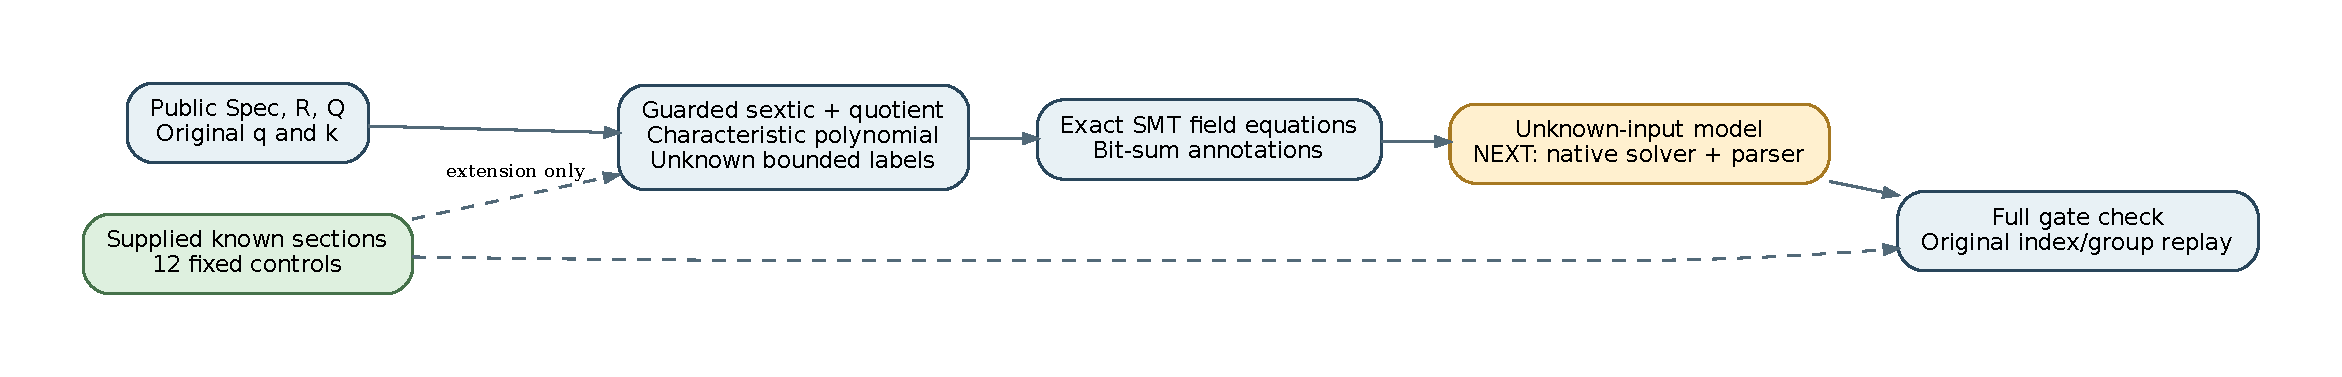
\includegraphics[width=\linewidth]{diagram.pdf}
\end{center}
\textbf{Backend admitted at interface scope.} The official cvc5 1.4.2 native
GPL/CoCoA release matches its published archive digest. Two scalar-root/model
checks over F101 and the actual prime field pass independent native scalar
replay. A 15-bit contradiction admits the bit-sum interface. No section system
was submitted to it, and no unknown coefficient root was discovered.
[pcc:PCC-20261123-989b50]

\textbf{Why BitSplit is a comparator.} Ozdemir et al., CAV 2024, split finite-field
equations into sparse and linear bases, separating bit sums from Boolean
constraints and refining conflicts. This fits the syntax of bounded label
words. The paper's exponential improvements concern verification, chiefly
unsatisfiable determinism queries. Its worst case still builds a full
Gr\"obner basis. Those results do not supply a decomposition-cost bound here.
No novelty is claimed for the established solver or algebraic primitives.

\textbf{Next concrete operation.} Parse all semantic model inputs strictly;
reconstruct and check every gate; then run unchanged numeric support and
original indexed/group extraction. Compare direct point and spectrum systems
on identical public targets under a separately frozen full-cost protocol.
Additional splitting of the quotient/Chebyshev and spectrum blocks needs its
own exact interface and projection check: ordinary BitSplit does not supply
that decomposition automatically. No search campaign or paid job is running.

\textbf{Acceptance remains separate.} Resource refusal, unknown, unsupported
extraction or unverified UNSAT is not target absence or a route disproof.
Useful target yield, growing-family work, setup/indexing/memory, row rank,
selection, kernel and recovery remain the original criteria's obligations.
The smaller export alone establishes no attack exponent. [pcc:unverified]

\textbf{Source map.} Native scope and raw subjects: PCC-20261123-989b50;
\texttt{PROTOCOL.md}, \texttt{SOURCE\_QUALIFICATION.json},
\texttt{native-v1/RETAINED\_BYTES.json}. Full native/compiler binding is open;
the earlier finite nilpotent Lean example retains its original limited scope.
The old malformed active record 8d8628 is retained with its correct companion
and erratum; this component does not change its gate standing.

\textbf{Primary references.} Ozdemir, Pailoor, Bassa, Ferles, Barrett, Dillig,
\emph{Split Gr\"obner Bases for Satisfiability Modulo Finite Fields}, CAV2024,
\href{https://theory.stanford.edu/~barrett/pubs/OPB+24.pdf}{author PDF},
\S\S3--5; \href{https://cvc5.github.io/docs/cvc5-1.4.2/theories/finite_field.html}{cvc5 finite-field reference}.
KB unavailable (wrapper127, no loaded connector); the repository assessment,
native source and primary paper/docs supplied the review. See \texttt{NEXT.md}.
\end{document}
